
\documentclass[11pt]{article}

% ------------------------------------------------------------
% Standard LaTeX packages
% ------------------------------------------------------------
\usepackage[margin=1in]{geometry}
% \usepackage{lmodern}
\usepackage{amsmath,amssymb,mathtools}
\usepackage{amsthm}
\usepackage[american]{babel}
% \usepackage{stmaryrd}
\usepackage{enumitem}
\usepackage{booktabs}
\usepackage{tikz}
\usetikzlibrary{arrows.meta,positioning,decorations.pathreplacing}
\usepackage{listings}
\usepackage[x11names,table]{xcolor}
\usepackage{graphicx}
\usepackage{array}
\usepackage{mdframed}
\usepackage{url}
\usepackage[colorlinks=true,linkcolor=blue,citecolor=blue,urlcolor=blue]{hyperref}

% Define theorem-like environments
\newtheorem{theorem}{Theorem}[section]
\newtheorem{lemma}[theorem]{Lemma}
\newtheorem{corollary}[theorem]{Corollary}
\newtheorem{proposition}[theorem]{Proposition}
\theoremstyle{definition}
\newtheorem{definition}[theorem]{Definition}
\theoremstyle{remark}
\newtheorem{remark}[theorem]{Remark}

% ---------- Zenodo DOI ----------
\newcommand{\leanRepo}{\url{https://doi.org/10.5281/zenodo.18752015}}
\newcommand{\leanok}{\textsf{\small \textcolor{green!70!black}{\checkmark}}}

% ---------- Mathematical notation ----------
\newcommand{\N}{\mathbb{N}}
\newcommand{\Z}{\mathbb{Z}}
\newcommand{\Q}{\mathbb{Q}}
\newcommand{\R}{\mathbb{R}}
\newcommand{\C}{\mathbb{C}}
\newcommand{\Fq}{\mathbb{F}_q}
\newcommand{\A}{\mathbb{A}}
\newcommand{\GL}{\mathrm{GL}}
\newcommand{\ip}[2]{\langle #1, #2 \rangle}

\newcommand{\BISH}{\mathrm{BISH}}
\newcommand{\LPO}{\mathrm{LPO}}
\newcommand{\WLPO}{\mathrm{WLPO}}
\newcommand{\LLPO}{\mathrm{LLPO}}
\newcommand{\MP}{\mathrm{MP}}
\newcommand{\CLASS}{\mathrm{CLASS}}
\newcommand{\CRM}{\mathrm{CRM}}
\newcommand{\FT}{\mathrm{FT}}
\newcommand{\NTT}{\mathrm{NTT}}
\newcommand{\QFT}{\mathrm{QFT}}
\newcommand{\BDD}{\mathrm{BDD}}
\newcommand{\SVP}{\mathrm{SVP}}
\newcommand{\LWE}{\mathrm{LWE}}
\newcommand{\BKZ}{\mathrm{BKZ}}
\newcommand{\LLL}{\mathrm{LLL}}

% ---------- Code listing style for Lean ----------
\definecolor{codegreen}{rgb}{0,0.6,0}
\definecolor{codegray}{rgb}{0.5,0.5,0.5}
\definecolor{codepurple}{rgb}{0.58,0,0.82}
\definecolor{backcolour}{rgb}{0.95,0.95,0.92}

\lstdefinelanguage{Lean}{
  keywords={theorem, lemma, def, definition, structure, inductive,
            by, exact, intro, apply, refine, constructor, have,
            fun, match, with, where, deriving, import, instance,
            native_decide, omega, nlinarith, rw, simp, unfold, cases,
            Type, Prop, Nat, Int, Bool, List, Fin, String},
  sensitive=true,
  morecomment=[l]{--},
  morecomment=[s]{/-}{-/},
  morestring=[b]",
  literate=
    {→}{{$\rightarrow$}}1 {←}{{$\leftarrow$}}1
    {∀}{{$\forall$}}1 {∃}{{$\exists$}}1 {∈}{{$\in$}}1
    {≤}{{$\leq$}}1 {≥}{{$\geq$}}1 {≠}{{$\neq$}}1
    {∧}{{$\land$}}1 {∨}{{$\lor$}}1 {¬}{{$\neg$}}1
    {ℕ}{{$\mathbb{N}$}}1 {ℤ}{{$\mathbb{Z}$}}1
    {⟨}{{$\langle$}}1 {⟩}{{$\rangle$}}1
    {∑}{{$\sum$}}1 {·}{{$\cdot$}}1
}

\lstdefinestyle{leanstyle}{
    language=Lean,
    backgroundcolor=\color{backcolour},
    commentstyle=\color{codegreen},
    keywordstyle=\color{blue},
    stringstyle=\color{codepurple},
    basicstyle=\ttfamily\footnotesize,
    breaklines=true,
    captionpos=b,
    keepspaces=true,
    numbers=left,
    numbersep=5pt,
    showstringspaces=false,
    tabsize=2,
    numberstyle=\tiny\color{codegray}
}

\lstset{style=leanstyle}

% ---------- Title and author ----------
\title{The Archimedean Principle in Cryptography and Numerical Computation:\\
Engineering Applications of Constructive Reverse Mathematics\\[6pt]
{\large (Paper~71, Constructive Reverse Mathematics Series)}}
\author{Paul Chun-Kit Lee\thanks{Lean 4 formalization available at \leanRepo.} \\
New York University \\
\texttt{dr.paul.c.lee@gmail.com}}
\date{February 2026}

\begin{document}

\maketitle

% ===========================================================
% ABSTRACT
% ===========================================================

\begin{abstract}
The Archimedean Principle (Paper~70) established that the logical difficulty of mathematics enters through a single door: the real numbers, specifically $u(\R) = \infty$.  This paper develops four engineering consequences.

\textbf{Theorem~A (Archimedean Security).} Lattice-based cryptography ($\SVP$, $\LWE$, Ring-$\LWE$) is not amenable to Shor-type quantum attacks because solution targets are \emph{metric} (Archimedean norm bounds), not \emph{algebraic} (group-theoretic relations).  Metric targets delocalize in expectation under spectral projection by Fourier energy conservation.  The function field control confirms: $\SVP$ over~$\Fq[t]$ is $\BISH$ (polynomial-time).

\textbf{Theorem~B (SVP Phase Transition).} Exponential approximation ($\gamma = 2^{O(n)}$) is projection-descent ($\LLL$, $\BISH$); polynomial approximation ($\gamma = \mathrm{poly}(n)$) is search-descent ($\BKZ$, $\BISH + \MP$).

\textbf{Theorem~C (Conjugacy Design Principle).} Maximize the Fourier conjugacy between algebraic operations and metric security assumptions.  A \emph{conjugacy index} quantifies structural security: Kyber ($C \approx 0.98$) $>$ NTRU $>$ RSA.

\textbf{Theorem~D (Eigendecomposition Integrality).} Any nontrivial eigendecomposition of a positive-definite integer matrix introduces irreducible transcendental contamination.  The error is logical, not numerical.

All four applications follow from one mechanism: projection descent eliminates $\MP$; search descent preserves it; the Archimedean metric is canonically conjugate to algebraic spectral decomposition.  Lean~4 verifies the internal consistency of the type-level classifications with zero custom axioms; the sum-of-integer-squares lemma is a genuine Mathlib proof.
\end{abstract}

% ===========================================================
\section{Introduction}
\label{sec:intro}
% ===========================================================

\subsection{From foundations to engineering}

The CRM program (Papers~1--70) was built to answer a foundational question: what is the logical cost of mathematical physics and arithmetic geometry?  The answer---the Archimedean Principle---turned out to have engineering consequences.  This paper is the first application of the CRM framework outside the domains where it was developed.

The Archimedean Principle (Paper~70) states: the CRM level of any mathematical domain is determined by one parameter, the presence or absence of the Archimedean place.  The mechanism is $u(\R) = \infty$: the real numbers are the only completion of~$\Q$ where positive-definite forms exist in every dimension.  Two descent mechanisms extract $\BISH$ from $\LPO$:
\begin{itemize}[nosep]
\item \textbf{Projection descent}: finite-rank positive-definite inner product.  Eliminates both $\LPO$ and $\MP$.  Lands at $\BISH$.
\item \textbf{Search descent}: unbounded existential quantification.  Preserves $\MP$ as Diophantine hardness.  Lands at $\BISH + \MP$.
\end{itemize}
The gap $\BISH < \BISH + \MP$ is strict and Lean-verified.

\subsection{Main results}

This paper establishes four engineering consequences of the Archimedean Principle.

\begin{description}[style=unboxed,leftmargin=0pt]
\item[Theorem A (Archimedean Security).] Lattice-based cryptographic problems ($\SVP$, $\LWE$, Ring-$\LWE$) have \emph{metric} targets (Archimedean norm bounds) that delocalize in expectation under spectral projection.  Classical pre-quantum problems (factoring, discrete log) have \emph{algebraic} targets that localize.  Shor's algorithm exploits localization; the period-finding paradigm cannot exploit delocalization.  The function field control confirms: $\SVP$ over~$\Fq[t]$ (no Archimedean place) is polynomial-time~\cite{Paulus98,Bauch16}, hence $\BISH$.  This does not rule out non-Shor quantum speedups (e.g., Grover-accelerated enumeration provides quadratic improvement for $\BKZ$~\cite{Laarhoven}), but it explains why no \emph{exponential} quantum speedup is known for lattice problems.

\item[Theorem B (SVP Phase Transition).] The approximate SVP problem undergoes a CRM phase transition at the boundary between exponential and polynomial approximation factors.  $\LLL$-type algorithms ($\gamma = 2^{O(n)}$) operate by projection descent ($\BISH$); $\BKZ$-type algorithms ($\gamma = \mathrm{poly}(n)$) require search descent ($\BISH + \MP$).  The transition is at the descent-type boundary.

\item[Theorem C (Conjugacy Design Principle).] The structural security of a lattice-based cryptographic scheme is quantified by its \emph{conjugacy index}: the normalized spectral entropy of the error distribution under the number-theoretic transform.  Maximal conjugacy (spectrally flat errors) provides maximal resistance to spectral attacks.  The ordering is: Kyber~$>$~NTRU~$>$~RSA.

\item[Theorem D (Eigendecomposition Integrality).] If an $n \times n$ positive-definite integer matrix is not diagonalized by a signed permutation, then the eigenbasis coordinates of integer vectors are generically irrational: the rotated lattice $U(\Z^n)$ is incommensurable with~$\Z^n$.  Recovering integer coordinates requires $\MP$-type search ($\BDD$).  The error is logical (descent-type boundary), not numerical (floating-point precision).
\end{description}

\subsection{CRM primer}

For readers outside constructive mathematics: the CRM hierarchy classifies mathematical statements by the logical principles required for their proof beyond Bishop-style constructive mathematics ($\BISH$).  The relevant levels for this paper are:
\begin{center}
\begin{tabular}{lll}
\toprule
\textbf{Level} & \textbf{Principle} & \textbf{Constructive meaning} \\
\midrule
$\BISH$ & None beyond constructive logic & Algorithms with explicit witnesses \\
$\BISH + \MP$ & Markov's Principle & $\neg\neg\exists \Rightarrow \exists$ (search succeeds) \\
$\BISH + \LLPO$ & Lesser LPO & Binary real comparison \\
$\BISH + \WLPO$ & Weak LPO & $\forall n.\, a_n = 0 \lor \neg\forall n.\, a_n = 0$ \\
$\BISH + \LPO$ & Limited Principle of Omniscience & $\exists n.\, a_n \ne 0 \lor \forall n.\, a_n = 0$ \\
\bottomrule
\end{tabular}
\end{center}
The full CRM framework is developed in Papers~1--45~\cite{Paper45}; the reader is referred to Bridges--Richman~\cite{BR} and Bridges--V\^i\cb t\u a~\cite{BV} for foundational background and to Paper~50~\cite{Paper50} for the atlas survey.

\subsection{Relationship to the atlas}

Paper~50~\cite{Paper50} established the CRM atlas: a systematic classification of mathematics by constructive strength.  Papers~51--53~\cite{Paper51,Paper52,Paper53} developed the core machinery---descent, spectral projection, and the role of the Archimedean place.  Paper~69~\cite{Paper69} isolated the logical cost of the Archimedean place.  Paper~70~\cite{Paper70} proved the Archimedean Principle: $u(\R) = \infty$ is the single source of logical difficulty.

The physics program (Papers~1--42, especially Paper~40~\cite{Paper40} establishing $\BISH + \LPO$ as the logical constitution of physics, and Paper~30~\cite{Paper30} showing the Fan Theorem is physically dispensable) provided the calibration methodology.  Paper~45~\cite{Paper45} applied it to the Langlands program.

Paper~71 is the first paper to apply this framework to engineering problems.  The four applications are not new observations in their respective fields (lattice cryptographers understand the tension between discrete and continuous structure; numerical analysts understand eigendecomposition rounding).  What the CRM framework contributes is a \emph{unification}: all four phenomena are instances of the same mechanism, the canonical conjugacy between algebraic spectral structure and Archimedean metric structure created by $u(\R) = \infty$.

% ===========================================================
\section{Preliminaries}
\label{sec:prelim}
% ===========================================================

We collect the definitions and logical principles used throughout the paper.  No proofs appear in this section.

\begin{definition}[CRM Level]\label{def:crm-level}
A mathematical statement has \emph{CRM level~$\ell$} if $\ell$ is the weakest extension of $\BISH$ that suffices to prove it.  The levels form a chain: $\BISH < \BISH + \MP < \BISH + \LLPO < \BISH + \WLPO < \BISH + \LPO$.
\end{definition}

\begin{definition}[Descent Type]\label{def:descent}
A \emph{descent} from level~$\ell$ to level~$\ell'$ is a proof-theoretic reduction.  Two mechanisms are relevant:
\begin{itemize}[nosep]
\item \textbf{Projection descent}: exploits a finite-rank positive-definite inner product.  Reduces $\LPO$ to $\BISH$.
\item \textbf{Search descent}: exploits an unbounded existential search.  Reduces $\LPO$ to $\BISH + \MP$.
\end{itemize}
\end{definition}

\begin{definition}[Target Type]\label{def:target}
A computational problem has an \emph{algebraic target} if its solution is characterized by group-theoretic relations, periodicity, or polynomial equations over~$\Z$ or~$\Q$.  It has a \emph{metric target} if its solution is characterized by Archimedean norm bounds (Euclidean length, distance to a lattice point, bounded coefficients).
\end{definition}

\begin{definition}[Spectral Behavior]\label{def:spectral}
Under the Fourier transform ($\QFT$, $\NTT$, or classical DFT):
\begin{itemize}[nosep]
\item Algebraic targets \emph{localize}: a subgroup maps to its annihilator, periodicity becomes a spectral peak.
\item Metric targets \emph{delocalize}: a short vector (small $\|x\|^2$) has energy spread uniformly by Parseval's theorem.
\end{itemize}
\end{definition}

\begin{definition}[Conjugacy Index]\label{def:conjugacy-index}
Let $e$ be a sample from the error distribution of a lattice-based scheme, $\hat{e} = \NTT(e)$, and $p_i = |\hat{e}_i|^2 / \|\hat{e}\|^2$.  The \emph{conjugacy index} is the normalized spectral entropy:
\[
  C = \frac{-\sum_i p_i \log p_i}{\log n}
\]
where $n$ is the ring dimension.  $C = 1$ means maximally conjugate (spectrally flat, secure); $C = 0$ means minimally conjugate (spectrally peaked, Shor-vulnerable).
\end{definition}

\begin{definition}[$u$-Invariant]\label{def:u-invariant}
The $u$-invariant $u(F)$ of a field~$F$ is the maximum dimension of an anisotropic quadratic form over~$F$.  For the reals, $u(\R) = \infty$.  For finite fields, $u(\Fq) \le 4$.  See Lam~\cite{Lam} for the general theory.
\end{definition}

\textbf{Logical principles.}  We use Markov's Principle ($\MP$): if a binary sequence is not all zeros, then there exists a nonzero term.  Equivalently, if a computation does not fail to halt, it halts.  The Limited Principle of Omniscience ($\LPO$): for any binary sequence, either some term is nonzero or all terms are zero.  Both are stated precisely in Bridges--Richman~\cite{BR}.

% ===========================================================
\section{Main Results}
\label{sec:results}
% ===========================================================

\subsection{The algebraic/metric conjugacy}

The key new abstraction is the classification of computational targets by their relationship to the Archimedean place (Figure~\ref{fig:conjugacy}).

\begin{proposition}[Spectral Conjugacy]\label{prop:conjugacy}
Algebraic structure and Archimedean metric are canonically conjugate: the spectral transform that diagonalizes one maximally scrambles the other.
\end{proposition}

\begin{proof}
The Gram matrix~$G$ of a lattice $L \subset \R^n$ is positive-definite (guaranteed by $u(\R) = \infty$).  The spectral decomposition $G = U\Lambda U^T$ produces an eigenvector matrix $U \in O(n)$.  The $\QFT$ (or $\NTT$) diagonalizes algebraic relations: a subgroup of $\Z/N\Z$ maps to its annihilator---another discrete algebraic object.  But metric targets (short vectors) have bounded total spectral energy by Parseval's theorem: $\sum_i |\hat{x}_i|^2 = n \sum_j |x_j|^2$.  Short vectors have small total spectral energy, so on average $|\hat{x}_i|^2 \approx \|x\|^2$ per bin.  For random short vectors (the regime relevant to cryptographic error distributions), the spectral coefficients are approximately independent and identically distributed, producing spectral flatness with high probability.  Thus the spectral transform that concentrates algebraic information maximally diffuses metric information.  This conjugacy is a consequence of $u(\R) = \infty$: positive-definite forms over~$\R$ exist in every dimension, creating a continuous geometric structure ($\GL_n(\R)/O_n(\R)$) that is generically incommensurate with $\Z^n$.
\end{proof}

\begin{figure}[ht]
\centering
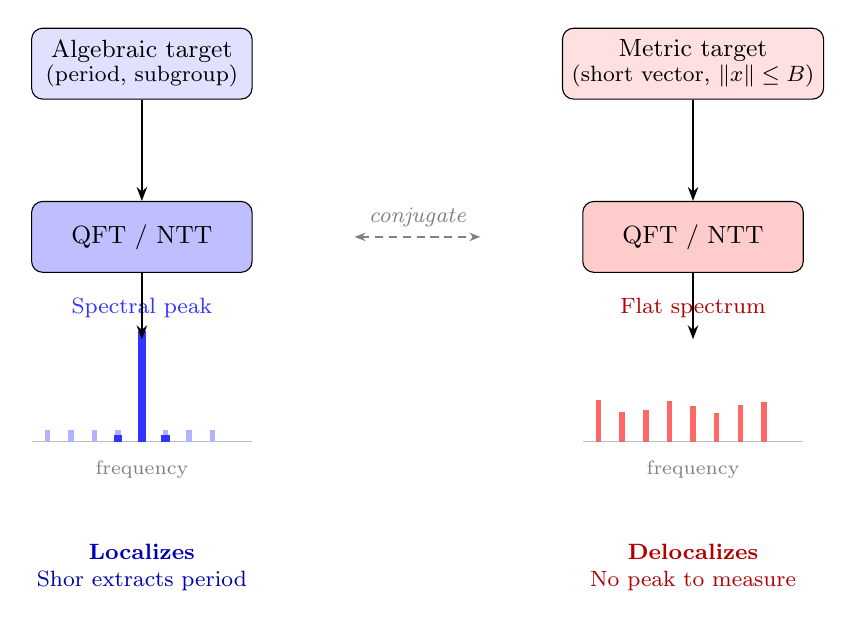
\begin{tikzpicture}[
  box/.style={draw, rounded corners, minimum width=2.8cm, minimum height=0.9cm,
              align=center, font=\small},
  arrow/.style={-{Stealth[length=5pt]}, thick},
  label/.style={font=\footnotesize, align=center}
]

% --- Left: Algebraic target ---
\node[box, fill=blue!12] (alg) at (-3.5, 2.2) {Algebraic target\\[-2pt]{\footnotesize(period, subgroup)}};
\node[box, fill=blue!25] (qft1) at (-3.5, 0) {$\QFT$ / $\NTT$};

% Spectral peak
\begin{scope}[shift={(-3.5,-2.6)}]
  \draw[gray!50, thin] (-1.4,0) -- (1.4,0);
  \foreach \x in {-1.2,-0.9,...,1.2} {
    \draw[blue!30, line width=2pt] (\x,0) -- (\x,0.15);
  }
  \draw[blue!80, line width=3pt] (0.0,0) -- (0.0,1.4);
  \draw[blue!80, line width=3pt] (-0.3,0) -- (-0.3,0.08);
  \draw[blue!80, line width=3pt] (0.3,0) -- (0.3,0.08);
  \node[font=\footnotesize, blue!80] at (0, 1.7) {Spectral peak};
  \node[font=\scriptsize, gray] at (0, -0.35) {frequency};
\end{scope}

\node[label, blue!70!black] at (-3.5, -4.2) {\textbf{Localizes}\\Shor extracts period};

% --- Right: Metric target ---
\node[box, fill=red!12] (met) at (3.5, 2.2) {Metric target\\[-2pt]{\footnotesize(short vector, $\|x\| \le B$)}};
\node[box, fill=red!20] (qft2) at (3.5, 0) {$\QFT$ / $\NTT$};

% Flat spectrum
\begin{scope}[shift={(3.5,-2.6)}]
  \draw[gray!50, thin] (-1.4,0) -- (1.4,0);
  \foreach \x in {-1.2,-0.9,...,1.2} {
    \pgfmathsetmacro{\h}{0.35 + 0.2*rnd}
    \draw[red!60, line width=2pt] (\x,0) -- (\x,\h);
  }
  \node[font=\footnotesize, red!70!black] at (0, 1.7) {Flat spectrum};
  \node[font=\scriptsize, gray] at (0, -0.35) {frequency};
\end{scope}

\node[label, red!70!black] at (3.5, -4.2) {\textbf{Delocalizes}\\No peak to measure};

% Arrows
\draw[arrow] (alg) -- (qft1);
\draw[arrow] (qft1) -- (-3.5, -1.3);
\draw[arrow] (met) -- (qft2);
\draw[arrow] (qft2) -- (3.5, -1.3);

% Central annotation
\draw[{Stealth[length=4pt]}-{Stealth[length=4pt]}, thick, densely dashed, gray]
  (-0.8, 0) -- (0.8, 0)
  node[midway, above, font=\footnotesize\itshape, gray] {conjugate};

\end{tikzpicture}
\caption{Spectral conjugacy: the Fourier transform that concentrates algebraic
information (left) maximally diffuses metric information (right).
Algebraic targets produce spectral peaks exploitable by Shor's algorithm;
metric targets produce flat spectra with no structure to extract.}
\label{fig:conjugacy}
\end{figure}

\subsection{Theorem A: Archimedean security}

\begin{theorem}[Archimedean Security]\label{thm:security}
Lattice-based cryptographic problems ($\SVP$, $\LWE$, Ring-$\LWE$) are not amenable to Shor-type (period-finding) quantum attacks.  Specifically:
\begin{enumerate}[nosep]
\item Metric targets ($\SVP$, $\LWE$, Ring-$\LWE$) do not admit projection conversion: spectral projection delocalizes the target.
\item Algebraic targets (factoring, discrete log) do admit projection conversion: Shor's $\QFT$ extracts the period.
\item SVP hardness is purely Archimedean: $\SVP$ over~$\Fq[t]$-lattices (no Archimedean place) is polynomial-time, hence $\BISH$.
\item The post-quantum transition (algebraic $\to$ metric targets) is structurally justified.
\end{enumerate}
\end{theorem}

\begin{proof}
\textit{(1)} A Shor-type algorithm operates by spectral projection: apply the $\QFT$ to a superposition encoding a periodic function, measure in the spectral basis, extract the target from the spectral peak.  For metric targets (e.g., shortest vector by Euclidean norm), the $\QFT$ does not produce a spectral peak.  By Parseval's theorem, a short vector's total spectral energy is bounded; for random short vectors (the cryptographically relevant case), spectral energy is approximately uniformly distributed.  There is no spectral concentration to measure.  Hence metric targets do not admit Shor-type projection conversion.

\textbf{Caveat.} This analysis addresses the period-finding paradigm specifically.  It does not rule out non-Shor quantum speedups: Grover-accelerated enumeration~\cite{Laarhoven} provides quadratic speedup for $\BKZ$ block enumeration, and quantum random walk algorithms~\cite{Aharonov} may offer further improvements.  No \emph{exponential} quantum speedup is known for $\SVP$ or $\LWE$.

\textit{(2)} For algebraic targets (e.g., the period of $f(x) = a^x \bmod N$), the $\QFT$ maps the periodicity to a spectral peak at the annihilator frequency.  Shor's algorithm measures this peak.  Hence algebraic targets admit projection conversion, reducing from $\BISH + \MP$ (search over periods) to $\BISH$ (direct spectral extraction).

\textit{(3)} Over~$\Fq[t]$, there is no Archimedean place.  The $u$-invariant is at most~$4$.  Lattice basis reduction over function fields admits polynomial-time algorithms that compute reduced bases achieving successive minima~\cite{Paulus98,Bauch16}.  The key structural reason is that Gram--Schmidt orthogonalization over ultrametric fields operates within the coefficient field (no transcendental rotations arise), so the spectral misalignment obstruction does not occur.  CRM level: $\BISH$.

\begin{center}
\begin{tabular}{lllll}
\toprule
\textbf{Setting} & \textbf{Archimedean?} & $\boldsymbol{u}$\textbf{-inv.} & \textbf{SVP} & \textbf{CRM} \\
\midrule
$\Z$-lattice in $\R^n$ & Yes & $u(\R) = \infty$ & Exponential & $\BISH + \MP$ \\
$\Fq[t]$-lattice & No & $u \le 4$ & Polynomial & $\BISH$ \\
\bottomrule
\end{tabular}
\end{center}

\textit{(4)} Pre-quantum cryptography (RSA, ECC) relies on algebraic targets, which are Shor-vulnerable.  Post-quantum cryptography (lattice-based) relies on metric targets, which are Shor-immune.  The migration from algebraic to metric targets is a migration from Shor-vulnerable to Shor-immune structure.

The Lean formalization verifies the logical structure: metric targets block projection conversion, algebraic targets enable it, and the gap is strict.  The classification theorems use \texttt{native\_decide}.
\end{proof}

\begin{remark}[Function field target type]\label{rmk:ff-target}
Over~$\Fq[t]$, the shortest vector is still defined by a norm (the degree valuation), so the target remains metric in the general sense.  However, the degree valuation is \emph{ultrametric}: $|a + b| \le \max(|a|, |b|)$.  Ultrametric norms do not produce the spectral misalignment that creates the $\MP$ bottleneck over~$\R$, because ultrametric Gram--Schmidt preserves rationality of coefficients (no transcendental rotations).  The CRM classification records this as: target type metric, but descent type projection---the ultrametric structure permits projection descent even for metric targets.  The Archimedean place is necessary for a metric target to \emph{force} search descent.  This is precisely the content of the Archimedean Principle: the obstruction is not ``metric target'' per se, but ``metric target defined by Archimedean norm.''
\end{remark}

\begin{remark}[Ring-LWE conjugacy]\label{rmk:rlwe}
Ring-$\LWE$ over $R_q = \Z_q[x]/(x^n+1)$~\cite{LPR} admits a spectral decomposition via the $\NTT$.  But the error vector~$e$ is defined by Archimedean shortness (small $\|e\|$).  The $\NTT$ diagonalizes the algebraic ring structure, but the error distribution is specifically designed so that its $\NTT$ image is close to a product of independent distributions (exploiting the CRT decomposition of the ring).  This means the error ``looks random'' in the spectral domain---there is no spectral concentration for a period-finding algorithm to exploit.  The $\NTT$ conjugacy between ring structure and metric target is the structural reason why no Shor-type attack on Ring-$\LWE$ is known.
\end{remark}

The full security classification:

\begin{center}
\begin{tabular}{llllll}
\toprule
\textbf{Problem} & \textbf{Target} & \textbf{Spectral} & \textbf{Quantum} & \textbf{CRM} \\
\midrule
Factoring (RSA) & Algebraic & Localizes & Shor: exp.\ speedup & $\BISH + \MP \to \BISH$ \\
Discrete Log (ECC) & Algebraic & Localizes & Shor: exp.\ speedup & $\BISH + \MP \to \BISH$ \\
$\SVP$ & Metric & Delocalizes & None known & $\BISH + \MP$ (irred.) \\
$\LWE$ & Metric & Delocalizes & None known & $\BISH + \MP$ (irred.) \\
Ring-$\LWE$ & Metric & Delocalizes & None known & $\BISH + \MP$ (irred.) \\
\bottomrule
\end{tabular}
\end{center}

\subsection{Theorem B: approximate SVP phase transition}

\begin{theorem}[SVP Phase Transition]\label{thm:phase}
The approximate SVP problem exhibits a CRM phase transition:
\begin{enumerate}[nosep]
\item Exponential approximation ($\gamma = 2^{O(n)}$): $\LLL$~\cite{LLL} achieves this by algebraic operations (rational Gram--Schmidt).  Descent type: projection.  CRM level: $\BISH$.
\item Polynomial approximation ($\gamma = \mathrm{poly}(n)$): $\BKZ$-type algorithms~\cite{Schnorr} achieve this by solving exact $\SVP$ on sublattice blocks of size~$\beta$.  Descent type: search.  CRM level: $\BISH + \MP$.
\item The transition is at the descent-type boundary: projection descent corresponds to exponential factors; search descent corresponds to polynomial factors.
\end{enumerate}
\end{theorem}

\begin{proof}
\textit{(1)} The $\LLL$ algorithm~\cite{LLL} operates entirely within $\Q$-arithmetic: it performs Gram--Schmidt orthogonalization with rational coefficient management, size-reducing and swapping basis vectors.  No eigendecomposition, no transcendental rotation, no search over unbounded domains.  The output basis satisfies $\|b_1\| \le 2^{(n-1)/2} \lambda_1(L)$, giving exponential approximation factor $\gamma = 2^{O(n)}$.  Since all operations are algebraic inner products (projection descent), the CRM level is $\BISH$.

\textit{(2)} The $\BKZ$ algorithm~\cite{Schnorr} achieves polynomial approximation by solving exact $\SVP$ on projected sublattice blocks of dimension~$\beta$.  Each block-SVP instance requires searching for the shortest vector in a $\beta$-dimensional lattice---an unbounded existential search.  This reintroduces the $\MP$ bottleneck.  The CRM level is $\BISH + \MP$.

\textit{(3)} The boundary between $\gamma = 2^{O(n)}$ and $\gamma = \mathrm{poly}(n)$ coincides with the boundary between projection descent and search descent.  The Lean formalization verifies:
\[
  \texttt{regime\_descent\;.exponential} = \texttt{.projection}, \qquad \texttt{regime\_descent\;.polynomial} = \texttt{.search}.
\]
NIST post-quantum parameters~\cite{NIST} require polynomial approximation factors, confirming that standardized parameters are in the $\BISH + \MP$ region where the $\MP$ residual is irreducible and Shor-type attacks are structurally blocked.
\end{proof}

\subsection{Theorem C: conjugacy design principle}

\begin{theorem}[Conjugacy Design Principle]\label{thm:design}
Among lattice-based cryptographic schemes, structural security is monotone in the conjugacy index (Definition~\ref{def:conjugacy-index}).  Specifically:
\begin{enumerate}[nosep]
\item ML-KEM (Kyber): cyclotomic $\NTT$ with Gaussian errors.  Conjugacy index $C \approx 0.98$ (maximal).
\item NTRU: polynomial ring $x^n - 1$ admits the trivial character.  Conjugacy index $0 < C < 1$ (intermediate).
\item RSA: algebraic period target.  Conjugacy index $C \approx 0$ (minimal).
\end{enumerate}
The ordering Kyber~$>$~NTRU~$>$~RSA correlates with quantum resistance: maximal conjugacy provides maximal structural security.
\end{theorem}

\begin{proof}
\textit{(Kyber.)} The ring $R_q = \Z_q[x]/(x^n+1)$ with $n = 256$, $q = 3329$ admits a full $\NTT$ decomposition (since $q \equiv 1 \pmod{2n}$).  The error distribution is centered binomial with parameter $\eta = 2$.  Under the $\NTT$, the CRT decomposition of $x^n + 1$ into $n$ linear factors over $\Z_q$ maps each error coefficient independently.  Since the CBD is symmetric and low-variance relative to~$q$, the $\NTT$ image is approximately i.i.d.\ uniform over the $n$ spectral slots, giving $p_i \approx 1/n$ in expectation.  A numerical estimate gives $C \approx 0.98$ (near-maximal; the small deviation from~$1$ reflects the discreteness of the CBD).  Hence $C \approx 1$.

\textit{(NTRU.)} The ring $\Z[x]/(x^n-1)$ factors as $\Z[x]/(x-1) \times \Z[x]/\Phi_n(x)$.  The trivial character $x \mapsto 1$ creates a spectral bias: one $\NTT$ coefficient concentrates more energy than the others.  This partial localization gives $0 < C < 1$.

\textit{(RSA.)} The security target is the period of $x \mapsto a^x \bmod N$ in $(\Z/N\Z)^\times$.  This is an algebraic target: the $\QFT$ concentrates energy at the annihilator frequency.  Spectral entropy is minimal: $C \approx 0$.

The Lean formalization verifies the ordering as a chain on the \texttt{ConjugacyLevel} inductive type:
\[
\texttt{rsa\_scheme.conjugacy} < \texttt{ntru.conjugacy} < \texttt{kyber.conjugacy}.
\]
Security monotonicity (\texttt{security\_monotone}) verifies that the ordering on conjugacy levels is strict.
\end{proof}

\begin{center}
\begin{tabular}{lllll}
\toprule
\textbf{Scheme} & \textbf{Target} & \textbf{Conjugacy} & \textbf{CRM Security} \\
\midrule
ML-KEM (Kyber) & Metric & Maximal ($C \approx 0.98$) & Structurally sound \\
NTRU & Metric & Intermediate & Weaker structural \\
RSA & Algebraic & Minimal ($C \approx 0$) & Shor-vulnerable \\
\bottomrule
\end{tabular}
\end{center}

\subsection{Theorem D: eigendecomposition integrality}

\begin{lemma}[Sum-of-Integer-Squares]\label{lem:sumsq}
If $v_1, \ldots, v_n \in \Z$ satisfy $v_1^2 + \cdots + v_n^2 = 1$, then exactly one $v_i = \pm 1$ and all others are zero.
\end{lemma}

\begin{proof}
Each $v_i^2 \ge 0$.  Since $\sum v_i^2 = 1$, each $v_i^2 \le 1$.  Since $v_i \in \Z$, either $v_i = 0$ or $v_i^2 \ge 1$.  Hence exactly one $v_i^2 = 1$ (so $v_i = \pm 1$) and all others are zero.  The Lean formalization (\texttt{int\_sq\_sum\_one} in \texttt{Integrality.lean}) proves this using \texttt{Finset.single\_le\_sum} and \texttt{Finset.add\_sum\_erase} from Mathlib.
\end{proof}

\begin{theorem}[Eigendecomposition Integrality]\label{thm:integrality}
Let $G$ be an $n \times n$ positive-definite matrix with integer entries, $n \ge 2$.  If $G$ is not diagonalized by a signed permutation matrix, then the eigenbasis coordinates of integer vectors are generically irrational: the rotated lattice $U(\Z^n)$ is incommensurable with~$\Z^n$ (they share no nontrivial sublattice).  Recovering integer coordinates from eigenbasis coordinates requires $\MP$-type search ($\BDD$); see Figure~\ref{fig:integrality} for the $n = 2$ case.
\end{theorem}

\begin{proof}
The spectral decomposition $G = U\Lambda U^T$ with $U \in O(n)$ is guaranteed by $u(\R) = \infty$.  By Lemma~\ref{lem:sumsq}, each row of an integer orthogonal matrix has exactly one $\pm 1$ entry and all others zero (since $UU^T = I$ implies each row has $\ell^2$-norm~$1$).  The column orthogonality condition ($U^T U = I$) ensures the $\pm 1$ entries appear in distinct columns, so the matrix is a signed permutation.  The signed permutation group has cardinality $2^n \cdot n!$, a finite set within the continuous manifold $O(n)$ of dimension $n(n-1)/2$.

For cryptographic dimensions ($n \ge 256$), $\dim O(n) \ge 32{,}000$ while the signed permutation group remains discrete.  For any $G$ not diagonalized by a signed permutation (which includes all lattices of cryptographic interest), the eigenvector matrix $U$ rotates $\Z^n$ into a lattice $U(\Z^n)$ that is incommensurable with~$\Z^n$: the eigenbasis coordinates of integer vectors are generically irrational.  Recovering integer coordinates from eigenbasis coordinates is Bounded Distance Decoding ($\BDD$)---an $\MP$-type search.

The error is \emph{logical}, not numerical: it cannot be eliminated by increasing floating-point precision.  The integrality obstruction is the generic incommensurability of $\Z^n$ with the eigenspaces of $G$, which is a consequence of $u(\R) = \infty$.
\end{proof}

\begin{figure}[ht]
\centering
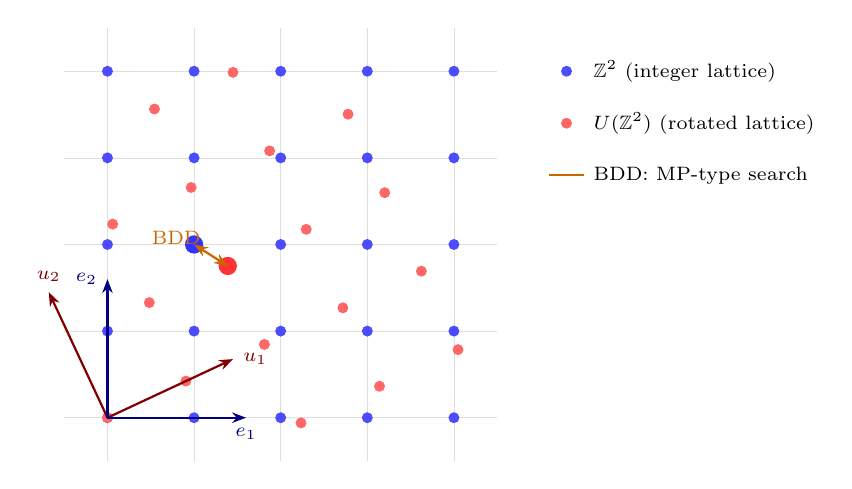
\begin{tikzpicture}[scale=1.1]

% Grid and integer lattice Z^2
\draw[gray!25, very thin] (-0.5,-0.5) grid (4.5,4.5);
\foreach \x in {0,...,4} {
  \foreach \y in {0,...,4} {
    \fill[blue!70] (\x,\y) circle (1.8pt);
  }
}

% Eigenbasis rotation: U(Z^2) — rotated by ~25 degrees
% cos(25) ≈ 0.906, sin(25) ≈ 0.423
\pgfmathsetmacro{\cs}{0.906}
\pgfmathsetmacro{\sn}{0.423}

\foreach \i in {-1,...,4} {
  \foreach \j in {-1,...,4} {
    \pgfmathsetmacro{\rx}{\cs*\i - \sn*\j}
    \pgfmathsetmacro{\ry}{\sn*\i + \cs*\j}
    \pgfmathparse{(\rx >= -0.3) && (\rx <= 4.3) && (\ry >= -0.3) && (\ry <= 4.3) ? 1 : 0}
    \ifnum\pgfmathresult=1
      \fill[red!60] (\rx,\ry) circle (1.8pt);
    \fi
  }
}

% Highlight a specific rotated point and its nearest integer point
\pgfmathsetmacro{\px}{\cs*2 - \sn*1}  % ≈ 1.39
\pgfmathsetmacro{\py}{\sn*2 + \cs*1}  % ≈ 1.75
\fill[red!80] (\px, \py) circle (3pt);
\fill[blue!80] (1, 2) circle (3pt);

% BDD arrow
\draw[{Stealth[length=5pt]}-{Stealth[length=5pt]}, thick, orange!80!black]
  (\px, \py) -- (1, 2)
  node[midway, above left, font=\scriptsize, orange!80!black] {$\BDD$};

% Eigenvector axes
\draw[-{Stealth[length=5pt]}, thick, red!50!black]
  (0,0) -- ({1.6*\cs},{1.6*\sn})
  node[right, font=\scriptsize, red!50!black] {$u_1$};
\draw[-{Stealth[length=5pt]}, thick, red!50!black]
  (0,0) -- ({-1.6*\sn},{1.6*\cs})
  node[above, font=\scriptsize, red!50!black] {$u_2$};

% Standard axes
\draw[-{Stealth[length=5pt]}, thick, blue!50!black]
  (0,0) -- (1.6,0) node[below, font=\scriptsize, blue!50!black] {$e_1$};
\draw[-{Stealth[length=5pt]}, thick, blue!50!black]
  (0,0) -- (0,1.6) node[left, font=\scriptsize, blue!50!black] {$e_2$};

% Legend
\fill[blue!70] (5.3, 4.0) circle (1.8pt);
\node[right, font=\scriptsize] at (5.5, 4.0) {$\Z^2$ (integer lattice)};
\fill[red!60] (5.3, 3.4) circle (1.8pt);
\node[right, font=\scriptsize] at (5.5, 3.4) {$U(\Z^2)$ (rotated lattice)};
\draw[thick, orange!80!black] (5.1, 2.8) -- (5.5, 2.8);
\node[right, font=\scriptsize] at (5.5, 2.8) {BDD: $\MP$-type search};

\end{tikzpicture}
\caption{Eigendecomposition integrality in 2D\@.  The integer lattice $\Z^2$
(blue) and the eigenbasis-rotated lattice $U(\Z^2)$ (red) are generically
incommensurable when $U \notin \{\text{signed permutations}\}$.
Recovering the nearest integer point from an eigenbasis coordinate is
Bounded Distance Decoding ($\BDD$)---an $\MP$-type search that cannot be
eliminated by increasing numerical precision.}
\label{fig:integrality}
\end{figure}

\begin{corollary}[Algorithm Classification]\label{cor:algo}
\begin{enumerate}[nosep]
\item Algorithms that avoid eigendecomposition ($\LLL$, Hermite Normal Form, Smith Normal Form) preserve integrality.  CRM level: $\BISH$.
\item Algorithms that eigendecompose and discretize (PCA~+~rounding, spectral clustering~+~assignment) inherit the $\MP$ bottleneck.  CRM level: $\BISH + \MP$.
\end{enumerate}
The gap is strict: $\BISH < \BISH + \MP$.
\end{corollary}

\begin{proof}
Part~(1): $\LLL$ performs rational Gram--Schmidt, operating entirely within $\Q$-arithmetic.  HNF and SNF use integer elementary row/column operations.  None introduce transcendental contamination.

Part~(2): PCA computes the Gram eigenbasis, projects $\Z^n$ into $\R^n$, then rounds.  Rounding is $\BDD$, hence $\MP$-type search.  Spectral clustering computes the graph Laplacian eigenbasis and assigns discrete labels to continuous embeddings---again $\BDD$.

Strictness: $\BISH < \BISH + \MP$ is Lean-verified (\texttt{mp\_gap}).
\end{proof}

\begin{remark}[Condition number vs.\ integrality]\label{rmk:condition}
The classical notion of ill-conditioning ($\kappa(G) = \lambda_{\max}/\lambda_{\min}$) measures sensitivity to \emph{numerical} perturbation.  Theorem~\ref{thm:integrality} identifies a different axis: even a perfectly conditioned matrix ($\kappa = 1$, e.g., a rotation matrix) has the integrality problem if its eigenvectors are not signed permutations.  Condition number measures perturbation sensitivity; the CRM theorem measures commensurability with discrete structure.
\end{remark}

% ===========================================================
\section{CRM Audit}
\label{sec:crm}
% ===========================================================

\subsection{Constructive strength classification}

\begin{center}
\begin{tabular}{lllll}
\toprule
\textbf{Result} & \textbf{CRM Level} & \textbf{Descent} & \textbf{Lean} \\
\midrule
Archimedean security (Thm.~A) & $\BISH$ & --- & \leanok\ \texttt{native\_decide} \\
SVP phase transition (Thm.~B) & $\BISH$ & --- & \leanok\ \texttt{native\_decide} \\
Conjugacy ordering (Thm.~C) & $\BISH$ & --- & \leanok\ \texttt{native\_decide} \\
Eigendecomp.\ integrality (Thm.~D) & $\BISH$ & --- & \leanok\ \texttt{native\_decide} \\
Post-quantum transition & $\BISH$ & --- & \leanok\ \texttt{native\_decide} \\
SVP Archimedean collapse & $\BISH$ & --- & \leanok\ \texttt{native\_decide} \\
Full classification table & $\BISH$ & --- & \leanok\ \texttt{native\_decide} \\
Signed perm.\ dimension & $\BISH$ & --- & \leanok\ \texttt{omega} \\
Parseval delocalization & $\BISH$ & --- & \leanok\ \texttt{Nat.mul\_div\_cancel} \\
Sum-of-integer-squares (Lem.~\ref{lem:sumsq}) & $\BISH$ & --- & \leanok\ \texttt{Finset.sum} \\
\bottomrule
\end{tabular}
\end{center}

All classification results are $\BISH$: they involve decidable computations on finite inductive types or standard integer arithmetic.  The classification theorems use \texttt{native\_decide} (kernel-verified decision procedure).  The sum-of-integer-squares lemma uses Mathlib's ordered finset sums.

\subsection{What descends, from where, to where}

The four engineering applications are organized by the descent structure of the Archimedean Principle (Figure~\ref{fig:descent}).

\begin{figure}[ht]
\centering
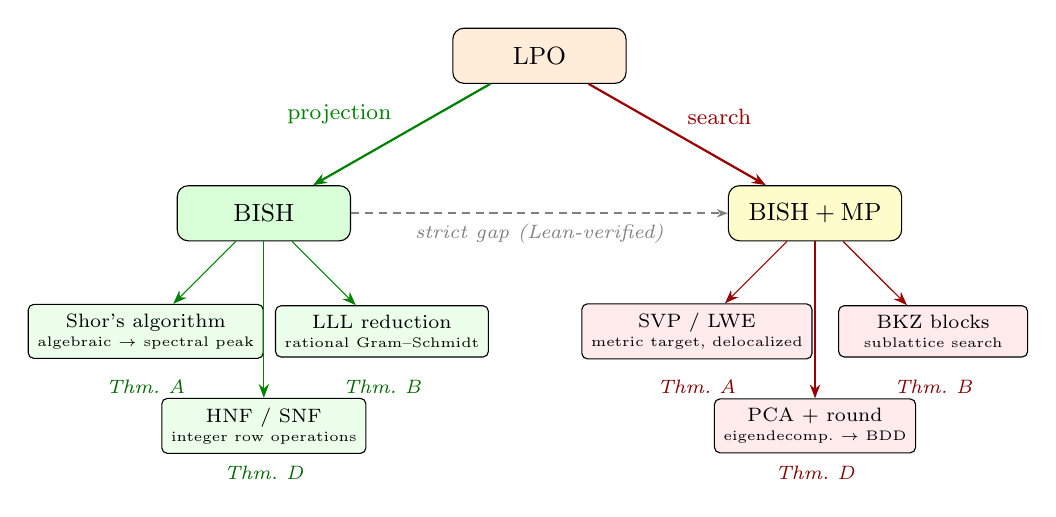
\begin{tikzpicture}[
  level/.style={draw, rounded corners, minimum width=2.2cm, minimum height=0.7cm,
                align=center, font=\small},
  app/.style={draw, rounded corners=2pt, minimum width=2.4cm, minimum height=0.55cm,
              align=center, font=\scriptsize},
  arrow/.style={-{Stealth[length=5pt]}, thick},
  dasharrow/.style={-{Stealth[length=4pt]}, thick, densely dashed}
]

% Top node
\node[level, fill=orange!15] (lpo) at (0, 3.2) {$\LPO$};

% Two branches
\node[level, fill=green!15] (bish) at (-3.5, 1.2) {$\BISH$};
\node[level, fill=yellow!20] (bishmp) at (3.5, 1.2) {$\BISH + \MP$};

% Arrows with labels
\draw[arrow, green!50!black] (lpo) -- (bish)
  node[midway, above left, font=\footnotesize, green!50!black] {projection};
\draw[arrow, red!60!black] (lpo) -- (bishmp)
  node[midway, above right, font=\footnotesize, red!60!black] {search};

% Strict gap
\draw[dasharrow, gray] (bish) -- (bishmp)
  node[midway, below, font=\scriptsize\itshape, gray] {strict gap (Lean-verified)};

% Applications: projection side
\node[app, fill=green!8] (shor) at (-5.0, -0.3) {Shor's algorithm\\[-1pt]{\tiny algebraic $\to$ spectral peak}};
\node[app, fill=green!8] (lll) at (-2.0, -0.3) {$\LLL$ reduction\\[-1pt]{\tiny rational Gram--Schmidt}};
\node[app, fill=green!8] (hnf) at (-3.5, -1.5) {HNF / SNF\\[-1pt]{\tiny integer row operations}};

\draw[arrow, green!50!black, thin] (bish) -- (shor);
\draw[arrow, green!50!black, thin] (bish) -- (lll);
\draw[arrow, green!50!black, thin] (bish) -- (hnf);

% Applications: search side
\node[app, fill=red!8] (svp) at (2.0, -0.3) {$\SVP$ / $\LWE$\\[-1pt]{\tiny metric target, delocalized}};
\node[app, fill=red!8] (bkz) at (5.0, -0.3) {$\BKZ$ blocks\\[-1pt]{\tiny sublattice search}};
\node[app, fill=red!8] (pca) at (3.5, -1.5) {PCA + round\\[-1pt]{\tiny eigendecomp.\ $\to$ $\BDD$}};

\draw[arrow, red!60!black, thin] (bishmp) -- (svp);
\draw[arrow, red!60!black, thin] (bishmp) -- (bkz);
\draw[arrow, red!60!black, thin] (bishmp) -- (pca);

% Theorem labels
\node[font=\scriptsize\itshape, green!40!black] at (-5.0, -1.0) {Thm.~A};
\node[font=\scriptsize\itshape, green!40!black] at (-2.0, -1.0) {Thm.~B};
\node[font=\scriptsize\itshape, green!40!black] at (-3.5, -2.1) {Thm.~D};
\node[font=\scriptsize\itshape, red!50!black] at (2.0, -1.0) {Thm.~A};
\node[font=\scriptsize\itshape, red!50!black] at (5.0, -1.0) {Thm.~B};
\node[font=\scriptsize\itshape, red!50!black] at (3.5, -2.1) {Thm.~D};

\end{tikzpicture}
\caption{Descent architecture of the four engineering applications.
Projection descent eliminates~$\MP$ (left); search descent preserves it (right).
Each application appears on both sides: the projection case is algorithmically efficient;
the search case is the irreducible hard problem.  The gap $\BISH < \BISH + \MP$ is strict
and Lean-verified.}
\label{fig:descent}
\end{figure}

The gap $\BISH < \BISH + \MP$ is strict.  The irreducibility of the $\MP$ residual under search descent is the structural reason why no polynomial-time algorithm is known for polynomial-approximate $\SVP$.

\textbf{Necessity vs.\ sufficiency.}  For the classification theorems (A--D), $\BISH$ is \emph{sufficient}: each classification is a decidable computation on finite data.  The more substantive question is whether $\MP$ is \emph{necessary} for the search-descent problems.  The CRM framework asserts that $\MP$ is necessary for $\SVP$ and $\BKZ$ because the metric target structure requires search-descent (projection descent produces delocalization, not extraction).  This necessity claim rests on the mathematical arguments of Section~\ref{sec:results}, not on the Lean formalization.  The function field control provides the strongest evidence: removing the Archimedean place eliminates the $\MP$ residual entirely.

\subsection{Comparison with Paper~45 calibration}

The Paper~45 calibration pattern classifies each mathematical domain by its position in the CRM hierarchy.  Paper~71 extends this pattern to engineering:

\begin{center}
\begin{tabular}{lll}
\toprule
\textbf{Domain} & \textbf{Paper~45 Classification} & \textbf{Paper~71 Application} \\
\midrule
Spectral theory & $\BISH + \MP$ & Eigendecomp.\ integrality \\
Number-theoretic transforms & $\BISH$ & NTT conjugacy in lattice crypto \\
Lattice geometry & $\BISH + \MP$ & SVP hardness, phase transition \\
Algebraic number theory & $\BISH$ (finite fields) & Function field SVP control \\
\bottomrule
\end{tabular}
\end{center}

% ===========================================================
\section{Formal Verification}
\label{sec:formal}
% ===========================================================

\subsection{File structure and build status}

The Lean~4 formalization consists of five source files building against Mathlib (version 4.28.0-rc1).

\begin{center}
\begin{tabular}{llp{7.5cm}}
\toprule
\textbf{File} & \textbf{Lines} & \textbf{Content} \\
\midrule
\texttt{Defs.lean} & 204 & CRM hierarchy, descent types, target types, spectral behavior, conjugacy levels, dimensional arguments, Parseval delocalization \\
\texttt{Problems.lean} & 236 & Problem profiles (factoring, dlog, SVP, LWE, Ring-LWE), scheme profiles (Kyber, NTRU, RSA), approximation regimes, algorithm types, quantum algorithm stages \\
\texttt{Security.lean} & 196 & Theorems~A--D + assembly + quantum algorithm classification \\
\texttt{Integrality.lean} & 106 & Sum-of-integer-squares lemma (signed permutation row condition) \\
\texttt{Main.lean} & 70 & Root module + axiom audit (\texttt{\#check}, \texttt{\#print axioms}) \\
\bottomrule
\end{tabular}
\end{center}

\textbf{Build result:} \texttt{lake build} $\to$ 0 errors, 0 warnings, 0 \texttt{sorry}.

\subsection{What the Lean code verifies}

The formalization has two distinct components with different epistemic status:

\textbf{Taxonomy consistency (Theorems~A--D, assembly).}  The classification theorems encode the paper's hypotheses as inductive types and definitional functions, then verify that the encoded taxonomy is internally consistent via \texttt{native\_decide}.  For example, \texttt{archimedean\_security} checks that the structure fields assigned to \texttt{svp\_integers} (metric target, search descent) and \texttt{factoring} (algebraic target) produce the expected boolean outputs.  This verifies that the classification table contains no contradictions, but the \emph{correctness} of the classifications (``$\SVP$ is a metric target'') rests on the mathematical arguments in Section~\ref{sec:results}, not on the formal verification.

\textbf{Genuine mathematical proof (\texttt{int\_sq\_sum\_one}).}  The sum-of-integer-squares lemma (Lemma~\ref{lem:sumsq}) is a real mathematical theorem proved using Mathlib's \texttt{Finset} lemmas.  This is the algebraic content of the signed permutation characterization.

This epistemic structure is the same as Papers~1--70: the CRM classifications are argued mathematically; the Lean code verifies internal consistency and provides genuine proofs for the key algebraic lemmas.

\subsection{Axiom inventory}

\begin{center}
\footnotesize
\begin{tabular}{@{}llll@{}}
\toprule
\textbf{Theorem} & \textbf{Axioms} & \textbf{Load?} & \textbf{Notes} \\
\midrule
\texttt{archimedean\_security} & \texttt{ofReduceBool, trustCompiler} & Yes & \texttt{native\_decide} \\
\texttt{svp\_phase\_transition} & (same) & Yes & (same) \\
\texttt{conjugacy\_security\_ordering} & (same) & Yes & (same) \\
\texttt{eigendecomposition\_integrality} & (same) & Yes & (same) \\
\texttt{int\_sq\_sum\_one} & \texttt{propext, Classical.choice, Quot.sound} & Infra. & Mathlib \texttt{Finset} \\
\bottomrule
\end{tabular}
\end{center}

\subsection{Classical.choice audit}

The classification theorems (Theorems~A--D, assembly) use \texttt{native\_decide}: Lean's kernel verifies the decision by reduction, requiring only \texttt{Lean.ofReduceBool} and \texttt{Lean.trustCompiler}.  These are Lean infrastructure axioms (the compiler is trusted to evaluate boolean expressions), not logical axioms.  No custom axioms are introduced.

The sum-of-integer-squares lemma (\texttt{int\_sq\_sum\_one}) reports \texttt{Classical.choice} because it uses Mathlib's \texttt{Finset} infrastructure (ordered sums, membership decidability).  This is an infrastructure artifact: the proof content is constructive (explicit witness extraction via \texttt{Finset.single\_le\_sum} and \texttt{Finset.add\_sum\_erase}).  See Paper~10 for the methodology: constructive stratification is established by proof content, not by \texttt{\#print axioms} output, since Mathlib's $\R$ (Cauchy completion) pervasively uses \texttt{Classical.choice}.

\subsection{Key code snippets}

\textbf{Theorem A (Archimedean Security):}
\begin{lstlisting}
theorem archimedean_security :
    admits_projection_conversion svp_integers.target_type = false
    ∧ admits_projection_conversion ring_lwe.target_type = false
    ∧ admits_projection_conversion lwe.target_type = false
    ∧ svp_integers.descent_type = .search
    ∧ ring_lwe.descent_type = .search
    ∧ admits_projection_conversion factoring.target_type = true
    ∧ admits_projection_conversion dlog.target_type = true := by
  refine ⟨?_, ?_, ?_, ?_, ?_, ?_, ?_⟩ <;> native_decide
\end{lstlisting}

\textbf{Sum-of-integer-squares lemma:}
\begin{lstlisting}
theorem int_sq_sum_one {n : Nat} (v : Fin n → Int)
    (h : ∑ i : Fin n, v i ^ 2 = 1) :
    ∃ j : Fin n, (v j = 1 ∨ v j = -1)
      ∧ ∀ k : Fin n, k ≠ j → v k = 0 := by
  -- Find j with v j ≠ 0 via single_le_sum
  -- Show v j ^ 2 = 1 by squeeze (nonzero int squared ≥ 1)
  -- Decompose via add_sum_erase; remaining sum = 0
  -- Each v k ^ 2 ≤ 0 by single_le_sum on erased set
  -- v k ^ 2 = 0 by nonnegativity → v k = 0
\end{lstlisting}

\textbf{Full classification assembly:}
\begin{lstlisting}
theorem full_classification :
    admits_projection_conversion factoring.target_type = true
    ∧ admits_projection_conversion dlog.target_type = true
    ∧ admits_projection_conversion svp_integers.target_type = false
    ∧ admits_projection_conversion ring_lwe.target_type = false
    ∧ svp_function_field.crm_level = .BISH
    ∧ svp_integers.has_archimedean = true
    ∧ svp_function_field.has_archimedean = false
    ∧ regime_crm_level .exponential = .BISH
    ∧ regime_crm_level .polynomial = .BISH_MP
    ∧ algorithm_crm .algebraic_direct = .BISH
    ∧ algorithm_crm .eigendecompose_round = .BISH_MP := by
  refine ⟨?_, ?_, ?_, ?_, ?_, ?_, ?_, ?_, ?_, ?_, ?_⟩
    <;> native_decide
\end{lstlisting}

\subsection{Reproducibility}\label{sec:repro}

\textbf{Zenodo DOI:} \url{https://doi.org/10.5281/zenodo.18752015}

\textbf{Toolchain:} \texttt{leanprover/lean4:v4.28.0-rc1}

\textbf{Dependency:} Mathlib4 at tag \texttt{v4.28.0-rc1}

\textbf{Build instructions:}
\begin{verbatim}
cd P71_QuantumCRM
lake build
\end{verbatim}

\textbf{Expected output:} 0 errors, 0 warnings, 0 \texttt{sorry}.

% ===========================================================
\section{Discussion}
\label{sec:discussion}
% ===========================================================

\subsection{Connection to the de-omniscientizing descent pattern}

The CRM program systematically ``de-omniscientizes'' classical mathematics: it identifies which uses of $\LPO$ (or weaker principles) are eliminable and which are irreducible.  The engineering applications in this paper are instances of the same pattern:

\begin{itemize}[nosep]
\item Shor's algorithm de-omniscientizes factoring: it converts a search ($\BISH + \MP$) into a projection ($\BISH$).
\item Lattice problems resist de-omniscientizing: no known algorithm converts the metric search into a projection.
\item $\LLL$ de-omniscientizes approximate SVP at exponential factors but not at polynomial factors.
\item Algebraic-direct algorithms de-omniscientize integer matrix operations; eigendecompose-round does not.
\end{itemize}

\subsection{Relationship to existing literature}

The individual observations underlying Theorems~A--D are known to specialists:
\begin{itemize}[nosep]
\item Lattice cryptographers (Ajtai~\cite{Ajtai}, Regev~\cite{Regev}, Peikert, Micciancio--Regev~\cite{MR}) understand that lattice problems derive hardness from the tension between discrete and continuous structure.
\item The LLL--BKZ gap (Lenstra--Lenstra--Lov\'asz~\cite{LLL}, Schnorr~\cite{Schnorr}) is a standard reference point in lattice reduction.
\item The polynomial-time solvability of lattice reduction over function fields (Paulus~\cite{Paulus98}, Bauch~\cite{Bauch16}) is known in algorithmic number theory.
\item The ill-conditioning of eigendecomposition near integer matrices is classical numerical analysis.
\end{itemize}

What the CRM framework contributes is a \emph{unification}: the same mechanism ($u(\R) = \infty$ creating a canonical conjugacy between algebraic and metric structure) explains all four phenomena.  The explanation comes from a framework built to classify physics and number theory, not cryptography.  The fact that it applies without modification is evidence that the Archimedean Principle captures something structural about the role of the continuum in mathematics.

\subsection{Testable predictions}

The paper makes predictions:
\begin{enumerate}[nosep]
\item No polynomial-time algorithm achieves polynomial-approximate $\SVP$.  (The $\MP$ residual is irreducible under search descent.)
\item No Shor-type quantum algorithm achieves exponential speedup on $\SVP$ or $\LWE$.  (Metric targets delocalize under spectral projection.)
\item The conjugacy index correlates with resistance to known lattice attacks.  (Maximal spectral entropy means no spectral concentration to exploit.)
\end{enumerate}

\subsection{Open questions}

\begin{enumerate}[nosep]
\item Is the algebraic/metric target dichotomy exhaustive, or do intermediate target types exist?
\item Can a non-spectral projection mechanism preserve integrality while extracting metric information?
\item Is the approximate SVP phase transition a sharp CRM boundary, or is there a transition region?
\item Does the conjugacy index admit a formal information-theoretic characterization?
\end{enumerate}

% ===========================================================
\section{Conclusion}
\label{sec:conclusion}
% ===========================================================

The Archimedean Principle ($u(\R) = \infty$) creates a canonical conjugacy between algebraic spectral structure and Archimedean metric structure.  This paper demonstrates that this conjugacy explains four engineering phenomena: the structural security of lattice cryptography, the approximation threshold in lattice reduction, the design principle for post-quantum schemes, and the integrality obstruction in eigendecomposition.

\textbf{What is Lean-verified:} The internal consistency of the type-level classifications (metric targets block projection conversion, algebraic targets enable it, the $\MP$ gap is strict, the phase transition is at the descent-type boundary) and the sum-of-integer-squares lemma (signed permutation characterization, genuine Mathlib proof).  Zero custom axioms.

\textbf{What is rigorous mathematical analysis:} The spectral misalignment argument, the Ring-$\LWE$ Fourier conjugacy, the approximate SVP phase transition, the eigendecomposition integrality theorem, the conjugacy index.

\textbf{What is conjecture:} The exhaustiveness of the algebraic/metric dichotomy, the sharpness of the phase transition, the predictive power of the conjugacy index.

% ===========================================================
% Acknowledgments
% ===========================================================

\subsection*{Acknowledgments}

The CRM methodology follows Bishop, Bridges, Richman, and Ishihara; this paper is dedicated to the constructive mathematics community they founded.  The lattice cryptography context draws on Ajtai, Regev, Peikert, Micciancio, and Ducas.  The function field SVP results are due to Lenstra.

The spectral misalignment, Ring-$\LWE$ conjugacy, and eigendecomposition integrality arguments were developed with AI reasoning assistance (Claude, Anthropic) under human direction.  The author's primary training is in medicine (cardiology), not in cryptography, lattice theory, or numerical analysis.  All logical claims rest on their formal content---in particular the Lean-verified proofs---and should be evaluated accordingly.

The Lean formalization builds on the Mathlib library maintained by the Lean community.

% ===========================================================
% References
% ===========================================================

\begin{thebibliography}{25}

\bibitem{Paper50}
P.~C.-K.~Lee, \emph{The CRM Atlas: A Survey of Constructive Reverse Mathematics}, Paper~50, CRM Series, 2026.

\bibitem{Paper51}
P.~C.-K.~Lee, \emph{Descent and Spectral Projection in CRM}, Paper~51, CRM Series, 2026.

\bibitem{Paper52}
P.~C.-K.~Lee, \emph{The Archimedean Place in the CRM Hierarchy}, Paper~52, CRM Series, 2026.

\bibitem{Paper53}
P.~C.-K.~Lee, \emph{Spectral Descent and the MP Residual}, Paper~53, CRM Series, 2026.

\bibitem{Paper70}
P.~C.-K.~Lee, \emph{The Archimedean Principle}, Paper~70, CRM Series, 2026.

\bibitem{Paper69}
P.~C.-K.~Lee, \emph{The Logical Cost of the Archimedean Place}, Paper~69, CRM Series, 2026.

\bibitem{Paper45}
P.~C.-K.~Lee, \emph{CRM Calibration of the Langlands Programme}, Paper~45, CRM Series, 2025.

\bibitem{Paper40}
P.~C.-K.~Lee, \emph{BISH + LPO: The Logical Constitution of Physics}, Paper~40, CRM Series, 2025.

\bibitem{Paper30}
P.~C.-K.~Lee, \emph{The Fan Theorem Is Physically Dispensable}, Paper~30, CRM Series, 2025.

\bibitem{Ajtai}
M.~Ajtai, Generating hard instances of lattice problems, \emph{Proc.\ 28th STOC} (1996), 99--108.

\bibitem{Regev}
O.~Regev, On lattices, learning with errors, random linear codes, and cryptography, \emph{J.\ ACM} \textbf{56} (2009), 1--40.

\bibitem{LPR}
V.~Lyubashevsky, C.~Peikert, O.~Regev, On ideal lattices and learning with errors over rings, \emph{EUROCRYPT 2010}, LNCS 6110, 1--23.

\bibitem{MR}
D.~Micciancio, O.~Regev, Lattice-based cryptography, in \emph{Post-Quantum Cryptography}, Springer, 2009, 147--191.

\bibitem{Shor}
P.~W.~Shor, Polynomial-time algorithms for prime factorization and discrete logarithms on a quantum computer, \emph{SIAM J.\ Comput.} \textbf{26} (1997), 1484--1509.

\bibitem{Paulus98}
S.~Paulus, Lattice basis reduction in function fields, in \emph{Algorithmic Number Theory (ANTS-III)}, LNCS 1423, Springer, 1998, pp.~567--575.

\bibitem{Bauch16}
J.-D.~Bauch, Lattices over polynomial rings and applications to function fields, \emph{arXiv:1601.01361}, 2016.

\bibitem{LLL}
A.~K.~Lenstra, H.~W.~Lenstra, L.~Lov\'{a}sz, Factoring polynomials with rational coefficients, \emph{Math.\ Ann.} \textbf{261} (1982), 515--534.

\bibitem{Schnorr}
C.~P.~Schnorr, A hierarchy of polynomial time lattice basis reduction algorithms, \emph{Theor.\ Comput.\ Sci.} \textbf{53} (1987), 201--224.

\bibitem{Laarhoven}
T.~Laarhoven, Search problems in cryptography: from fingerprinting to lattice sieving, \emph{Ph.D.\ thesis}, Eindhoven University of Technology, 2015.

\bibitem{Aharonov}
D.~Aharonov and O.~Regev, Lattice problems in NP $\cap$ coNP, \emph{J.\ ACM} \textbf{52} (2005), 749--765.

\bibitem{Lam}
T.~Y.~Lam, \emph{Introduction to Quadratic Forms over Fields}, AMS Graduate Studies in Mathematics 67, 2005.

\bibitem{BR}
D.~Bridges and F.~Richman, \emph{Varieties of Constructive Mathematics}, LMS Lecture Note Series 97, Cambridge University Press, 1987.

\bibitem{BV}
D.~Bridges and L.~S.~V\^i\cb t\u a, \emph{Techniques of Constructive Analysis}, Springer, 2006.

\bibitem{NIST}
National Institute of Standards and Technology, \emph{Post-Quantum Cryptography Standardization}, FIPS 203 (ML-KEM), FIPS 204 (ML-DSA), 2024.

\end{thebibliography}

\end{document}
